\chapter{EKF-SLAM Implementation}
\label{ch:chapter2}
In Chapter~\ref{ch:chapter1} the EKF-SLAM algorithm in the context of \ac{SLAM} was explained. As mentioned in Section~\ref{sec:chapter1:kf}, the algorithm can be summarized in two steps: prediction and correction. In the first stage involves the prediction of the next state of the system, meanwhile, during the correction stage, this estimation is updated. However, differently from the Algorithm~(\ref{alg:chapter1:slam:ekfslam}), the proposed implementation adds a \ac{NEES} test with th objective of improving the consistency of the filter. The updated version of the algorithm can be seen in Algorithm~(\ref{alg:chapter2:implementation:ekfslam}).\\
\begin{algorithm}[h]
    \caption{EKF-SLAM algorithm with NEES test}
    \label{alg:chapter2:implementation:ekfslam}
    \BlankLine
    \KwIn{$\mu_{t-1}$, $\Sigma_{t-1}$, $u_t$, $z_t$}
    \BlankLine
    $\hat\mu_t = g\left(\mu_{t-1}, u_t\right)$\;
    $G_t = computeJacobian\left(g\right)$\;
    $\hat\Sigma_t = G_t \Sigma_{t-1} G_t^T + R_t$\;
    \BlankLine
    \ForEach{landmark observation $z_t^i$}{
        \BlankLine
        \If{landmark $i$ has not being seen before}{
            $addLandmarkToStateVector\left( z_t^i \right)$
        }
        \BlankLine
        $H_t^i = computeJacobian\left( h^i \right)$\;
        $v^i =  z_t^i - h^i \left( \hat\mu_t \right)$\;
        $S = H_t^i \hat\Sigma_t H_t^{iT} + Q_t$\;
        $K_t^i = \hat\Sigma_t H_t^{iT} S^{-1}$ \;
        $e = {v^i}^T S^{-1} {v^i}$\;
        \If{$e < \chi_{\alpha}^2$}{
            $\mu_t = \hat\mu_t + K_t^i \left( v^i \right) $ \;
            $\Sigma_t = (I - K_t^i H_t^i) \hat\Sigma_t$ \;
        }
    }
    \BlankLine
    \Return{$\mu_t$, $\Sigma_t$}
\end{algorithm}

Line 11, computes the \ac{NEES} value, and line 12 compares it with the $\chi^2$ value for the specific landmark. If the \ac{NEES} value is lower than the $\chi^2$ threshold, the observation is accepted and the state vector and covariance matrix are updated.\\

In this chapter, an EKF-SLAM implementation is shown, starting from the used drone characteristics, going through the motion and observation models, visual process pipeline, and ending with the overall system's architecture.

\section{The Drone}
\label{sec:chapter2:drone}
\subsection{Characteristics}
\label{subsec:chapter2:drone:characteristics}
The drone considered for this analysis has a common characteristics, such as four rotors disposed as an X. The drone frame is called 3DR Iris Quadrotor, and can be seen in Figure~\ref{fig:chapter2:drone:frame}.

\begin{figure}
    \centering
    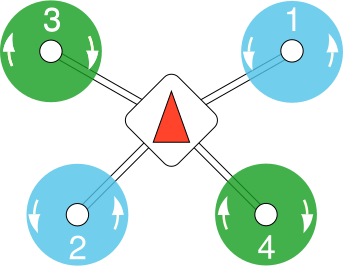
\includegraphics[width=0.5\textwidth]{Images/fig4-quad-frame.png}
    \caption[3DR Iris Quadrotor frame.]{3DR Iris Quadrotor frame \cite{mavros}.}
    \label{fig:chapter2:drone:frame}
\end{figure}

\subsubsection{Flight Controller}
The flight controller used in this case is a PixHawk 4, and its characteristics are shown in Table~\ref{tab:chapter2:drone:px4fc}. It is worth mentioning that it includes an integrated accelerometer, a gyroscope, a magnetometer and a barometer.

\begin{table}
    \centering
    \begin{tabular}{cp{27em}}
        \toprule \textsc{Item} & \textsc{Description}\\
        \midrule
        \multirow{2}{*}{Main FMU processor} & STM32F765 \\
        & 32 Bit Arm® Cortex®-M7, 216MHz, 2MB memory, 512KB RAM \\
        \midrule
        \multirow{2}{*}{IO Processor} & STM32F100 \\
        & 32 Bit Arm® Cortex®-M3, 24MHz, 8KB SRAM \\
        \midrule
        \multirow{4}{*}{On-board sensors} & Accel/Gyro: ICM-20689 \\
        & Accel/Gyro: BMI055 \\
        & Magnetometer: IST8310 \\
        & Barometer: MS5611 \\
        \midrule
        GPS & ublox Neo-M8N GPS/GLONASS receiver; integrated magnetometer IST8310 \\
        \midrule
        \multirow{10}{*}{Interfaces} & 8-16 PWM outputs (8 from IO, 8 from FMU) \\
        & 3 dedicated PWM/Capture inputs on FMU \\
        & Dedicated R/C input for CPPM \\
        & Dedicated R/C input for Spektrum / DSM and S.Bus with analog / PWM RSSI input \\
        & Dedicated S.Bus servo output \\
        & 5 general purpose serial ports \\
        & 3 I2C ports \\
        & 4 SPI buses \\
        & Up to 2 CANBuses for dual CAN with serial ESC \\
        & Analog inputs for voltage / current of 2 batteries \\
        \midrule
        \multirow{3}{*}{Power System} & Power module output: 4.9~5.5V \\
        & USB Power Input: 4.75~5.25V \\
        & Servo Rail Input: 0~36V \\
        \midrule
        \multirow{2}{*}{Weight and Dimensions} & Weight: 15.8g \\
        & Dimensions: 44x84x12mm \\
        \midrule
        Operating temperature & -40 to 85°c \\
        \bottomrule
    \end{tabular}
    \caption[PixHawk 4 Specification]{Technical specification of the PixHawk 4 flight controller.}
    \label{tab:chapter2:drone:px4fc}
\end{table}

\subsubsection{Additional Sensors}
The drone was equipped with several sensors that are the input for localization, mapping and path planning algorithms, among others.\\

The localization and mapping algorithm makes use, in an indirect way, of monocular and stereo cameras, and range sensors. Four cameras were mounted in order to be able to have 360 range view, with cameras mounted every 90 degrees. Furthermore, two stereo cameras were mounted, one points forward in order to update the Octomap and the other points downwards in order to see the markers; Also, both of them are used to build a 3-dimensional map, used for obstacle avoidance and with the height estimation algorithm. Furthermore, eight range sensors were mounted every 45 degrees, and one PIX4Flow optical flow camera points downwards in order to measure the distance to the ground.

\subsection{Reference Frames}
\label{subsec:chapter2:drone:frames}
This system is composed by three reference frames linked with each other, as represented in Figure~\ref{fig:chapter2:drone:frames:frames}: \emph{map}, \emph{odom} and \emph{base\_link}. The \emph{map} frame, also called \emph{world} or \emph{global} frame, is the static reference frame, where the global drone's position and global markers' position is set. The odom reference frame is similar to the map frame, but the difference is that this frame drifts with time, as happens with the pure odometry. Finally, the base\_link frame, also referred as \emph{body} or \emph{local} frame, refers to the center of mass of the drone.\\

As mentioned before, all transformations within these reference frames are published by different nodes: the map to odom transformation is handled by the \emph{rtabmap} node, the odom to base\_link is handled by \emph{mavros} node. There are many other transformations in the system, but they are mainly related to the base\_link reference frame and the different cameras and sensors in the drone. \\
\begin{figure}[h]
    \centering
    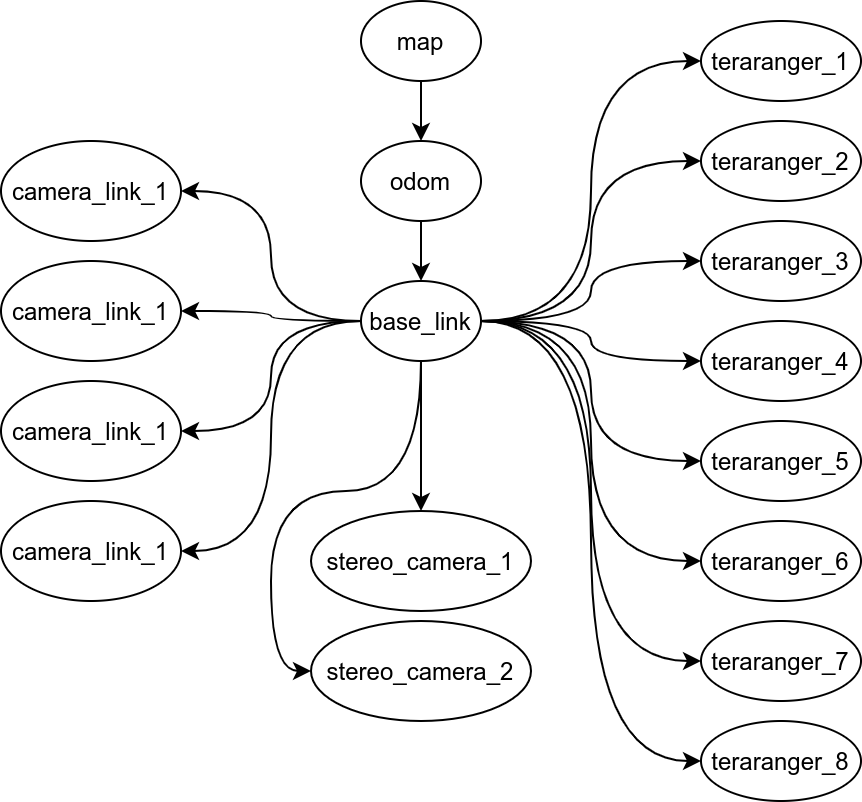
\includegraphics[width=0.7\textwidth]{Images/fig5-frames.png}
    \caption{Main reference frames in the system.}
    \label{fig:chapter2:drone:frames:frames}
\end{figure}

Finally, there is a transformation that worth mentioning: the \ac{NED} to \ac{ENU}. As mentioned in Section~\ref{sec:chapter1:ros}, \ac{ROS} uses the \ac{ENU} convention, while the convention adopted by the Aerospace community is the \ac{NED}. Also, as mentioned in Section~\ref{sssec:chapter2:drone:mavlink}, MAVROS is in charge of doing and publish this transformation. In Figure~\ref{fig:chapter2:drone:frames:enu2ned} a simple scheme of the transformation can be seen. As explained before, this transform consists on rotating the X-axis and the Y-axis by 90 degrees, hence the homogeneous rotation matrix will have the following form:
\begin{align}
    R_{ENU}^{NED} & = \begin{bmatrix}
        0 & -1 & 0 & 0 \\
        0 & 0 & 1 & 0 \\
        -1 & 0 & 0 & 0 \\
        0 & 0 & 0 & 1
    \end{bmatrix}
\end{align}


\begin{figure}
    \centering
    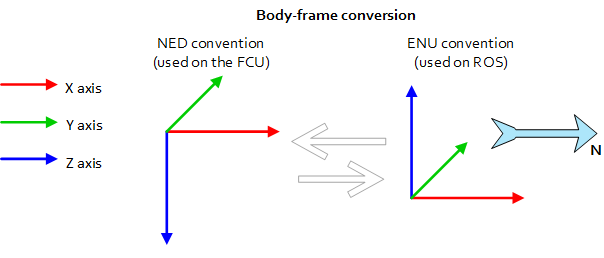
\includegraphics[width=\textwidth]{Images/fig6-ned2enu.png}
    \caption[NED to ENU conversion scheme]{\ac{NED} to \ac{ENU} conversion scheme. \cite{mavros}}
    \label{fig:chapter2:drone:frames:enu2ned}
\end{figure}

\section{Motion Model}
\label{sec:chapter2:prediction}
During the prediction step, the motion model and the covariance matrix update are computed. The motion model will update the state vector, which will store the position X, Y and Z in the global reference frame, and the orientation in the Z-axis of the drone. Fortunately MAVROS provides a node that makes odometry estimation based on different sensors outputs. The messages published by the odometry node, of type \inlinesrc{Odometry}, provide the linear velocity, the angular velocity and pose information. The velocity information is used to estimate the position in X, Y and Z, and the drone's orientation along the Z-axis. However, the velocity estimation provided by MAVROS is relative to the body reference frame, and this has to be transformed into the world reference frame, so before estimating the global position of the drone it is mandatory to do this transformation.

\begin{align}
    u &= \begin{bmatrix} v_x^b & v_y^b & v_z^b & \omega_x^b & \omega_y^b & \omega_z^b & \phi^b & \theta^b & \psi^b \end{bmatrix}^T\\
    v^w &= \textbf{T} * \begin{bmatrix} v_x^b \\ v_y^b \\ v_z^b \end{bmatrix}
\end{align}
where the control vector $u$ is composed by the linear velocities in the body reference frame ($v_x^b$, $v_y^b$, $v_z^b$), the angular velocities in the body reference frame ($\omega_x^b$, $\omega_y^b$, $\omega_z^b$) and the drone's orientation ($\phi^b$, $\theta^b$, $\psi^b$). Additionally, $\textbf{T}$ is the homogeneous transform (see Section~\ref{sec:chapter1:transform}) using the current orientation of the drone: $\phi^b$, $\theta^b$ and $\mu_{\psi}$. Notice the third element of the orientation ($\mu_{\psi}$), this is because the orientation over the Z-axis is estimated by the filter. As result, $v^w$ will be a column vector with the linear velocities in the global reference frame. \\

Given this, the motion model update can be summarized in the following calculation:
\begin{align}
    \hat\mu &=
    \begin{bmatrix}
        \mu_{t-1, x^w} \\ \mu_{t-1, y^w} \\ \mu_{t-1, z^w}
    \end{bmatrix}
    + \Delta t * v^w \\
    \hat\mu_{\psi} &= \mu_{t-1, \psi} + \Delta t * \omega_z^b
\end{align}

Then, $\textbf{G}_t$, which is the Jacobian matrix of the motion model, should be computed. As mentioned in Section~\ref{subsec:chapter1:slam:ekfslam}, it has the following characteristic:
\begin{align}
    G_t &= \begin{bmatrix}
        G_r & \textbf{0} \\
        \textbf{0} & \textbf{I}
    \end{bmatrix}\\
    G_r &= \begin{bmatrix}
        1 & 0 & 0 & G_{r, 14} \\
        0 & 1 & 0 & G_{r, 24} \\
        0 & 0 & 1 & 0 \\
        0 & 0 & 0 & 1
    \end{bmatrix}
\end{align}
\begin{align*}
     G_{r, 14} &= -\Delta t * (v_y^w * (c_{\phi} * c_{\psi} + s_{\theta} * s_{\phi} * s_{\psi}) - v_z^w * (c_{\psi} * s_{\phi} - c_{\phi} * s_{\theta} * s_{\psi}) + v_x^w * c_{\theta} * s_{\psi}) \\
     G_{r, 24} &= -\Delta t * (v_z^w * (c_{\psi} * s_{\phi} + c_{\phi} * s_{\theta} * c_{\psi}) -v_y^w * (c_{\phi} * s_{\psi} - s_{\theta} * s_{\phi} * c_{\psi}) + v_x^w * c_{\theta} * s_{\psi})
\end{align*}
where
\begin{alignat*}{3}
    c_{\phi} &= \cos{\left(u_{\phi}\right)}, \quad & c_{\theta} &= \cos{\left(u_{\theta}\right)}, \quad & c_{\psi} &= \cos{\left(\mu_{\psi}\right)} \\
    s_{\phi} &= \sin{\left(u_{\phi}\right)}, \quad & s_{\theta} &= \sin{\left(u_{\theta}\right)}, \quad & s_{\psi} &= \sin{\left(\mu_{\psi}\right)}
\end{alignat*}\\
The function $g$ that models the motion of the drone is assumed to be perfect and therefore noise free. So, before computing the covariance update, it is necessary to compute the process noise covariance matrix ($R_t$) that encodes the motion model noise which, in this case, is related to the underlying dynamics of the drone flight. The noise is assumed to be additive and Gaussian, and therefore, the motion model can be decomposed as:
\begin{equation}
    x_t = g(u_t, x_{t-1}) + \mathcal{N}\left(0, R_t\right)
    \label{eq:chapter2:prediction:motion_w_noise}
\end{equation}
\begin{equation}
    R_t = N * U * N^T
    \label{eq:chapter2:prediction:control_cov}
\end{equation}
the noise part in equation (\ref{eq:chapter2:prediction:motion_w_noise}) relates to the acceleration component that is, in this case, unknown. However, it is known from a theoretical perspective: the acceleration component in an accelerated movement is $\frac{1}{2}\Delta t^2 a$, where $a$ is the body's acceleration. Given this, we can assume that the noise component in the motion model is:
\begin{equation}
    \mathcal{N}\left(0, R_t\right) = \frac{1}{2} \Delta t^2 T_w^b \begin{bmatrix}
        a_x \\ a_y \\ a_z \\ a_{\psi}
    \end{bmatrix}
\end{equation}
where $T_w^b$ is the transformation matrix from body to world reference frame. The covariance of the process noise ($R_t$) can be decompose as shown in equation~(\ref{eq:chapter2:prediction:control_cov}), where matrix $N$ is the Jacobian of acceleration term  with respect to the state vector, and matrix $U$ is the estimated average acceleration.
\begin{equation}
    N = \frac{\partial \frac{1}{2} \Delta t^2 T_w^b \textbf{a}}{\partial \mu}
\end{equation}
\begin{equation}
    U = \textbf{I} * \begin{bmatrix}
        a_{avg, x} \\ a_{avg, y} \\ a_{avg, z} \\ a_{avg, \psi}
    \end{bmatrix}
\end{equation}
The multiplication in equation (\ref{eq:chapter2:prediction:control_cov}) provides an approximate mapping between the motion noise in control space and the motion noise in the state space.\\

Finally, the covariance update should be computed as follow
\begin{align}
    \hat\Sigma &= G_t * \Sigma * G_t^T + R_t
\end{align}

\section{Observation Models}
\label{sec:chapter2:correction}
While the drone is moving around the environment it senses different landmarks that may be included or not in the state vector. These observations will eventually improve the localization of the drone, and will improve the landmarks' poses if needed. The whole process involves the computation of the Jacobian of the observation model for the seen landmark, the computation of the Kalman gain, and the update of the state vector and covariance matrix.\\

To perform the correction step, EKF-SLAM needs a linearized observation model with additive Gaussian noise. In the case studied in this work, there are two kinds of landmarks and, therefore, two different observation models. The main difference between these two type of landmarks, is that the position of poles type is known, while it is not known in the case of markers. Hence, every time the robot "sees" a pole, the algorithm will update the drone's pose and the known markers' pose; while every time it "sees" a marker two course of action are possible:
\begin{enumerate}[a)]
    \item{if the marker is not known, it is added to the state vector, enlarging it along with the covariance matrix.}
    \item{if the marker is known, its pose, the pose of all other markers, and the drone's pose are updated.}
\end{enumerate}

The observation model is, as with the motion model in equation~(\ref{eq:chapter2:prediction:motion_w_noise}), assumed to be perfect and with an additive Gaussian noise. The noise here is related to the observation process, and so, related to the used sensors.
\begin{equation}
    z_i = h_i\left(x_t\right) + \mathcal{N}\left(0, Q_t\right)
    \label{eq:chapter2:correction:obs_w_noise}
\end{equation}
Consequently, the noise covariance matrix of the observation model cannot be deducted as with the noise covariance matrix of the motion model. In this case, the matrix should be constructed empirically based on the sensors' characteristics, and it has the following characteristic:
\begin{equation}
    Q_t = \begin{bmatrix}
        \sigma_1^2 &  & \textbf{0} \\
         & \ddots & \\
        \textbf{0} & & \sigma_n^2 \\
    \end{bmatrix}
\end{equation}\\
where the diagonal elements $\sigma_{1..n}$ are the standard deviation of the sensor. Depending on the sensor used, the diagonal elements can be the standard deviation for the range and bearing components (distance, azimuth and elevation), or others.\\

As shown in Algorithm~(\ref{alg:chapter1:slam:ekfslam}) and Algorithm~(\ref{alg:chapter2:implementation:ekfslam}) several steps are followed during the correction part of the algorithm. After computing the observation model and its Jacobian matrix, the Kalman gain and the innovation should be calculated, and finally, the state vector and covariance matrix updates should be done.

\subsection{Observation model for Poles}
\label{subsec:chapter2:correction:poles}
In the case of Poles, a range and bearing method is used. In this case, since the poles have a known position, their information is not kept in the state vector and therefore, this information will be used for localization purposes.\\

A \ac{ROS} node will publish the range and bearing information every time the drone sees a pole, and this information will be used to calculate the innovation based on the predicted range and bearing. Hence, the observation model used for poles is computed in the following way:
\begin{equation}
    \begin{bmatrix}
        p_{i, x}^b \\ p_{i, y}^b \\ p_{i, z}^b
    \end{bmatrix} = \bm{T_r}^{-1} \begin{bmatrix}
        p_{i, x}^w \\ p_{i, y}^w \\ p_{i, z}^w
\end{bmatrix}
\label{eq:chapter2:correction:pole:world2body_transform}
\end{equation}
\begin{equation}
    h_i(\hat\mu_t) = \begin{bmatrix}
        p_{i, \rho} \\ p_{i, \alpha} \\ p_{i, \beta}
    \end{bmatrix} = \begin{bmatrix}
    \sqrt{ p_{j, x^b}^2 + p_{j, y^b}^2 } \\
    \atantwo{p_{j, y}^b}{p_{j, x}^b} \\
    \atantwo{p_{j, z}^b}{p_{j,\rho}^b}
\end{bmatrix}
\label{eq:chapter2:correction:pole:range_bearing}
\end{equation}

In equation~(\ref{eq:chapter2:correction:pole:world2body_transform}), $\bm{T_r}^{-1}$ corresponds to the inverse of the homogeneous transformation matrix with respect to the current drone's pose, and elements $p_i^w$ are the $x$, $y$ and $z$ coordinates of the $i$ pole's tip in the world reference frame. This way, the global position of the pole $i$ is projected to the body reference frame. After that, the range ($\rho$), azimuth angle ($\alpha$) and elevation angle ($\beta$) are calculated, as shown in equation~(\ref{eq:chapter2:correction:pole:range_bearing}). In Figure~\ref{fig:chapter2:correction:poles:range_bearing} an example of the range and bearing is shown.
\begin{figure}[h]
    \centering
    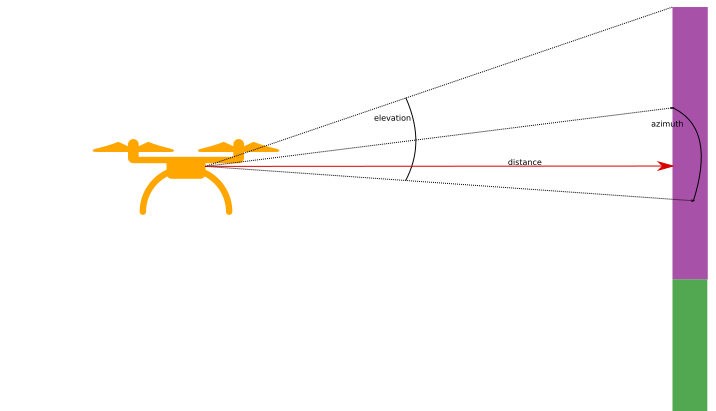
\includegraphics[width=\textwidth]{Images/fig7-range_and_bearing}
    \caption[Range and Bearing example]{Range and bearing example. The drone observes a pole, process the data from the sensors and estimates the distance ($\rho$), the elevation angle ($\beta$), and the azimuth angle ($\alpha$). The elevation angle is calculated based on the top extreme of the pole.}
    \label{fig:chapter2:correction:poles:range_bearing}
\end{figure}

Observing a pole affects only the drone's pose, and therefore, the Jacobian matrix of the observation model will have the following form:
\begin{equation}
    H_i = \begin{bmatrix}
        \frac{\partial \rho'}{\partial \mu_x} & \frac{\partial \rho'}{\partial \mu_y} & \frac{\partial \rho'}{\partial \mu_z} & \frac{\partial \rho'}{\partial \mu_{\psi}} & \dots & 0 \\
        \frac{\partial \alpha'}{\partial \mu_x} & \frac{\partial \alpha'}{\partial \mu_y} & \frac{\partial \alpha'}{\partial \mu_z} & \frac{\partial \alpha'}{\partial \mu_{\psi}} & \dots & 0 \\
        \frac{\partial \beta'}{\partial \mu_x} & \frac{\partial \beta'}{\partial \mu_y} & \frac{\partial \beta'}{\partial \mu_z} & \frac{\partial \beta'}{\partial \mu_{\psi}} & \dots & 0
    \end{bmatrix}
\end{equation}
where $\rho'$ corresponds to the distance part of the observation model, $\alpha'$ is the azimuth part, and $ \beta'$ the elevation part. The elements after the \nth{4} column are all 0, which means, as said before, that the observation of a pole will not affect the pose of the markers.

\subsection{Observation model for Markers}
\label{subsec:chapter2:correction:markers}

The observation model for the markers is a bit different. In this case a \ac{ROS} node is responsible of detecting, tracking and publishing the pose of the markers with respect to the camera that has seen it. The \ac{ROS} package responsible of this process is called \inlinesrc{visp_auto_tracker}, and publishes messages of type \inlinesrc{PoseStamped}, which provides the position and orientation of the seen marker. An example of this situation can be seen in Figure~\ref{fig:chapter2:correction:markers:example}.\\

\begin{figure}
    \centering
    \includegraphics[width=\textwidth]{Images/fig8-marker_example}
    \caption[Example of the drone observing a marker]{Example of the drone observing a marker. The camera visualize a marker and the node \inlinesrc{visp_auto_tracker} estimates its pose with respect to the camera reference frame.}
    \label{fig:chapter2:correction:markers:example}
\end{figure}

Every time the camera that points down sees a known marker, the \inlinesrc{visp_auto_tracker} node will publish the pose of that marker. This published pose is with respect to the camera which is not positioned at the drone's center of mass and so, a different transformation is needed. This process can be seen in equation~(\ref{eq:chapter2:correction:markers:world2body_trasnform}), in which the transformation of the marker's pose in the world reference frame is transformed to the pose in the camera reference frame.
\begin{equation}
    \begin{bmatrix}
        m_{i, x}^c \\ m_{i, y}^c \\ m_{i, z}^c \\ m_{i, \phi}^c \\ m_{i, \theta}^c \\ m_{i, \psi}^c
    \end{bmatrix} = (\bm{T_r} * \bm{T_c})^{-1} * \bm{T_m}
    \label{eq:chapter2:correction:markers:world2body_trasnform}
\end{equation}
where, $\bm{T_r}$ is the homogeneous transformation matrix of the drone's pose, $\bm{T_c}$ is the homogeneous transformation matrix of the camera's pose, and $\bm{T_m}$ is the homogeneous transformation of the marker's pose. The result is a vector that contains the marker's pose in the camera reference frame.\\

As mentioned before, observing a marker will update the drone's pose and that marker's pose, and therefore the Jacobian matrix of the observation model will have a different aspect from the pole's case. Here, the Jacobian can be split in two parts as shown in equation~(\ref{eq:chater2:correction:markers:jacobian}), where the left part, as with the poles, affects the drone's pose, while the right part of the matrix affects the seen marker's pose.
\begin{align}
    H_i &= \begin{bmatrix}
        \frac{\partial h_i(\hat\mu)}{\partial \mu_r} & \dots0\dots & \frac{\partial h_i(\hat\mu)}{\partial \mu_{m_i}} & \dots0\dots
    \end{bmatrix}
    \label{eq:chater2:correction:markers:jacobian}
\end{align}

The Jacobian matrices of the observation model with respect to the drone state and with respect the marker pose can be seen in \cite{polibri-github}. It is worth to mention that the reason why this matrix only contains two sections different to zero is because of the relations between markers: observing a marker does not affect the pose of others, and therefore, the Jacobians of the observation model for marker $i$ with respect to marker $i+1$ or any other marker is 0.\\

Furthermore, unlike the case of poles, the markers' pose is unknown the first time, and therefore the algorithm will introduce their pose into the state vector when the drone sees a previously unknown marker.

\subsubsection{Adding new Markers}
\label{subsubsec:chapter2:correction:markers:add}
%\nocite{slam-auto-mob-robots}
As mentioned in Section~\ref{subsec:chapter1:slam:ekfslam:addlandmarks}, to add new landmarks to the state vector an inverse observation model is needed. In the current case, the inverse observation model will project the observed marker's pose from the camera reference frame to the world reference frame. Equation~\ref{eq:chapter2:correction:markers:inverseh} shows the inverse observation model for markers where, similarly to the observation model, a set of transformations are performed but, this time, in order to obtain the pose of the seen marker in the world reference frame:
\begin{align}
    \begin{bmatrix}
        m_{i, x}^w \\ m_{i, y}^w \\ m_{i, z}^w \\ m_{i, \phi}^w \\ m_{i, \theta}^w \\ m_{i, \psi}^w
    \end{bmatrix} &= \bm{T_r} * \bm{T_c} * \bm{T_m}
    \label{eq:chapter2:correction:markers:inverseh}
\end{align}

As before, $\bm{T_r}$ is the homogeneous transformation matrix of the drone's pose, $\bm{T_c}$ is the homogeneous transformation matrix of the camera's pose, and $\bm{T_m}$ is the homogeneous transformation of the marker's pose. The result is a vector containing the marker's pose in the world reference frame, and with which will extend the state vector:
\begin{align*}
    \mu_t = \left[\begin{array}{c|cccccc}
        \mu_t & m_{i, x}^w & m_{i, y}^w & m_{i, z}^w & m_{i, \phi}^w & m_{i, \theta}^w & m_{i, \psi}^w
    \end{array}
    \right]^T
\end{align*}

Furthermore, the covariance matrix should be updated in order to contain the newly added marker. As shown in equation~\ref{eq:chapter1:slam:ekfslam:cov_update}, the Jacobian of the inverse observation model with respect to the drone's state and the Jacobian of the inverse observation model with respect to the marker's state are needed. Both Jacobian matrices can be seen in Appendix~\ref{appendix:a}. In this case, the matrix $\bm{Y_x}$ has a size of ($\norm{\mu}+6) \times (\norm{\mu})$ where $\norm{\mu}$ is the size of the state vector before adding the projected pose of the seen marker. On the other hand, the matrix $\bm{Y_z}$ has a size of $(\norm{\mu}+6) \times 6$. Given these two matrices, the new covariance matrix $\Sigma$ will be increased by 6 columns and 6 rows and will have the following form:
\begin{align*}
    \Sigma = \begin{bmatrix}
        \Sigma_{r,r} & \Sigma_{r,m} \\ \Sigma_{r,m} & \Sigma_{m,m}
    \end{bmatrix}
\end{align*}
where $\Sigma_{r,r}$ is the covariance matrix between the drone's state variables, the $\Sigma_{r,m}$ and $\Sigma_{m,r}$ is the covariance matrix between the drone and the markers' state variables, and between the markers and the drone's state variables, and $\Sigma_{m,m}$ is the covariance matrix between markers' state variables.

\subsection{Observation model for range sensor and height correction}
\label{subsec:chapter2:correction:range}
With respect to the height estimation, it is corrected by poles, markers and with a combination of PIX4Flow camera and Octomap. Both poles and markers update the altitude of the drone, but this estimation can be improved by using the optical flow camera and the Octomap generated by the stereo camera.\\

The Octomap is build with obstacle avoidance in mind, but it can be used jointly with the optical flow to correct the drone's Z position. To do so, the it can be assumed that the range sensor provided by the PIX4Flow camera, plus the Octomap voxel height below the camera should be equal to the drone's height. Hence, the range sensor model can be defined as:
\begin{equation}
    h\left(\hat\mu_t\right) = \hat\mu_z + bias
\end{equation}
and the observation is defined by:
\begin{equation}
    \hat{z} = voxel_z + range_{distance}
\end{equation}
where $voxel_z$ is the Z position of the voxel below the drone, and $range_{distance}$ is the sensed distance provided by the range sensor.\\

Hopefully, the Jacobian is a vector composed by zeroes except for the component related to the Z position of the drone:
\begin{equation}
    H = \begin{bmatrix}
        0 & 0 & 1 & \dots0\dots
    \end{bmatrix}
\end{equation}

Since the observation model is composed by a single variable, the Jacobian is a row vector of the size of the current state vector.


\section{Visual process pipeline}
\label{sec:chapter2:visual}
As mentioned in Section~\ref{sec:chapter2:drone}, the drone is composed by several cameras, specifically, two stereo cameras and four monocular cameras. These cameras are used to identify and avoid obstacles and for localization purposes. The localization process involves the identification of poles and markers, and therefore, the usage of the before mentioned cameras: the four monocular cameras are used to identify poles, while one stereo camera is used to identify the markers.
\subsection{Visual process for Poles}
Four \ac{ROS} nodes are responsible of determining whether a pole is being seen or not. To do so, they subscribe to topics related to the camera information and the camera image, and every time a new image arrives, each node process it to identify a pole. Each pole is composed by two different colors, and each pole has a different combination of colors making possible to uniquely identify them. The overall process can be followed in Algorithm~(\ref{alg:chapter2:visual_pipeline:poles}).\\
\begin{algorithm}[h]
    \caption{Poles localization algorithm}
    \label{alg:chapter2:visual_pipeline:poles}
    \BlankLine
    \KwIn{\inlinesrc{image_raw}, \inlinesrc{camera_info}}
    \BlankLine
    Apply masks to image\\
    Identify how many poles are in the image\\
    \If{contours of poles where found}{
        \ForEach{pole contour}{
            Find coordinates of contour\\
            Identify pole\\
            \If{the full width of the pole can be seen}{
                Compute Azimuth ($\alpha$)

                \If{the pole is not occluded}{
                    Compute Range ($\rho$)

                    \If{the top of the pole can be seen}{
                        Compute Altitude ($\beta$)
                    }
                }
            }
        }
    }
    \BlankLine
    \Return{$\alpha$, $\beta$, $\rho$}
\end{algorithm}

Lines 1 and 2, applies a mask in order to identify the amount of poles contours in the image. If there are pole contours in the image, at lines 5 and 6 the algorithm uniquely identifies the pole and its coordinates. If the width of the identified pole can be seen, at line 8 the algorithm computes the azimuth angle ($\alpha$) by using the drone's yaw and the center of the contour. At line 9, it estimates the probability of occlusion of the pole by comparing the contour shape with the form factor, computed as $\frac{y_{max} - y_{min}}{x_{max} - x_{min}}$ where $y_{max}$ and $y_{min}$ are the bottom and the top coordinates of the contour, and $x_{max}$ and $x_{min}$ are the right and left coordinates of the contour. If the probability is greater that 75\%, the range is computed based on the diameter of the contour. Finally, if the top of the contour can be seen (line 11), at line 12 it computes the altitude.

\subsection{Visual process for Markers}
The markers detection pipeline is performed by the \ac{ViSP} tracking package \cite{visp-paper}. The package wraps an automated pattern-based tracker based on \ac{ViSP} library, which allows to estimate an object pose with respect to the camera. In the case of this work a QR code is used as marker, which is identified by the tracker. \\

The \inlinesrc{visp_auto_tracker} node subscribes to the camera image and information topics, and publishes the detected object's pose. The camera messages are provided by the stereo camera that points downwards.

\section{Overall Architecture}
\label{sec:chapter2:arch}
The system is composed by several \ac{ROS} nodes that specialize and perform a wide range of operations. However, what is most interesting for this work is the node that is in charge of the EKF-SLAM process. \\

\begin{figure}
    \centering
    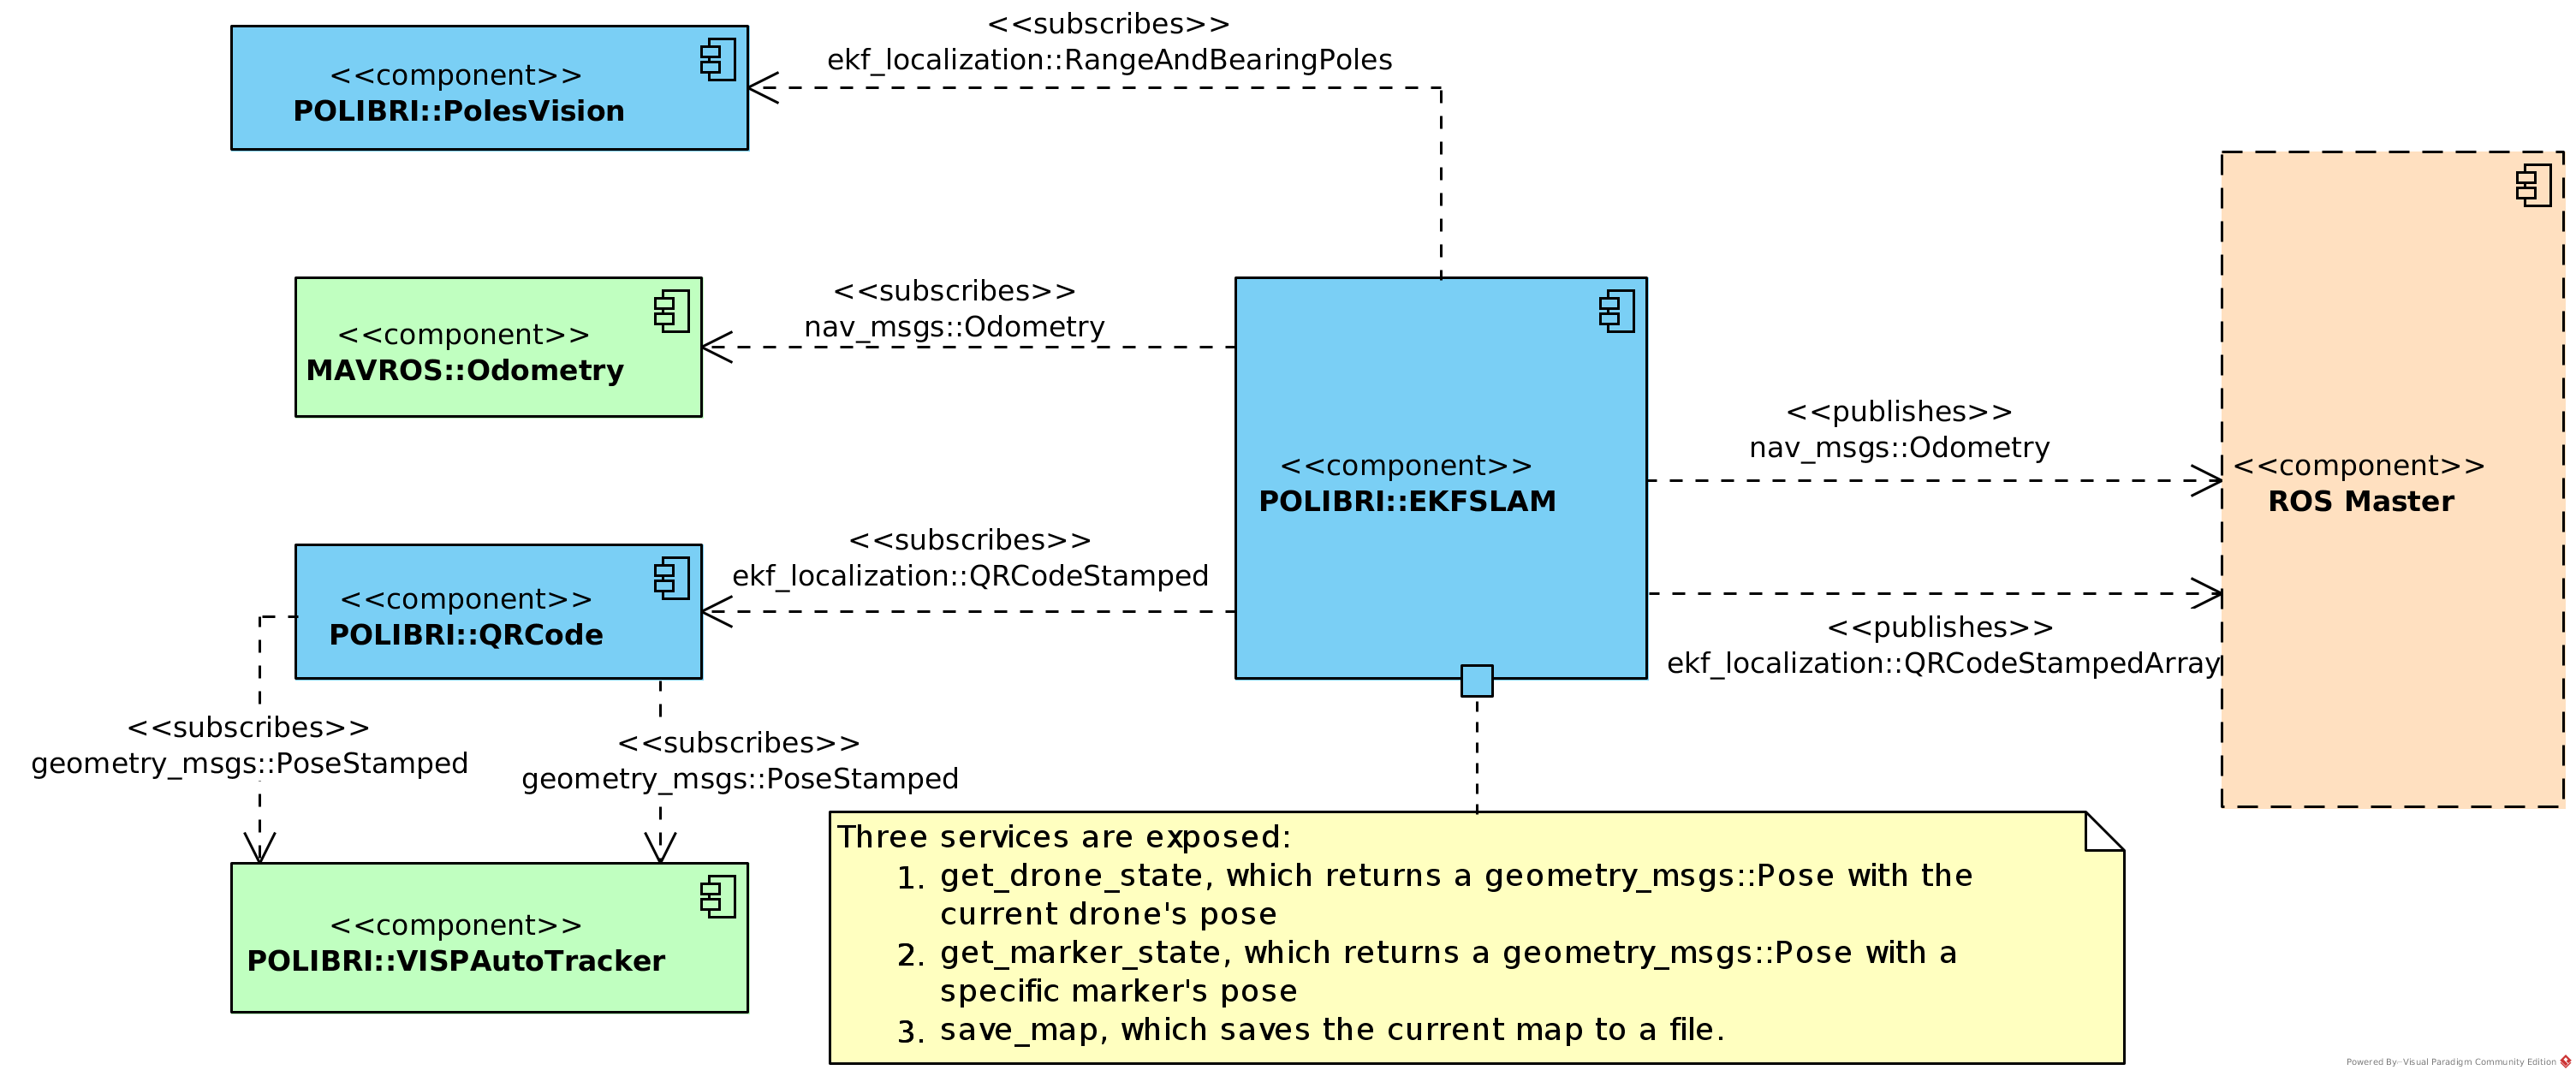
\includegraphics[width=\textwidth]{Images/fig9-components_diagram}
    \caption[Components diagram of the EKF Localization node]{Components diagram of the \ac{EKF} Localization node. The \inlinesrc{EKFSLAM} class subscribes to different messages, between them the \inlinesrc{Odometry} messages are used as control variables, while the \inlinesrc{RangeAndBearingPole} and \inlinesrc{QRCodeStamped} messages are used every time the drone observes a pole or a marker. Moreover, \inlinesrc{EKFSLAM} class publishes two types of messages: \inlinesrc{Odometry} which provides the filtered localization and \inlinesrc{QRCodeStampedArray} which contains a list markers' poses.}
    \label{fig:chapter2:architecture:components}
\end{figure}

In Figure~\ref{fig:chapter2:architecture:components} the components that interact around the \ac{EKF} Localization node can be seen. In the center of the figure the \inlinesrc{EKFSLAM} component is placed, which is responsible of running the EKF-SLAM algorithm. Every time an \inlinesrc{Odometry} message arrives, the prediction step takes place, and this happens every 30Hz. Furthermore, every time a \inlinesrc{RangeAndBearingPoles} or a \inlinesrc{QRCodeStamped} arrives the correction step takes place, and differently to the prediction step, this depends on whether the drone observes or not a pole or a marker. Additionally, the \inlinesrc{EKFSLAM} component provides three services:
\begin{enumerate}
    \item \inlinesrc{get_drone_state}: takes no arguments, and returns the current localization of the drone \inlinesrc{Pose} message.
    \item \inlinesrc{get_marker_state}: takes as argument the id of a marker, and returns the current estimated pose of that marker\inlinesrc{Pose} message.
    \item \inlinesrc{save_map}: takes no arguments, and it saves the current map in a YAML file. The map contains the pose of all the poles and all the markers seen so far.
\end{enumerate}

It is worth to mention that the messages of type \inlinesrc{QRCodeStamped} are provided by the \inlinesrc{QRCode} node which is internal to the \inlinesrc{ekf_localization} package. This node is needed because the \inlinesrc{visp_auto_tracker}, responsible of identifying the markers and publish their poses, publish these data as separate messages: the marker's id as a \inlinesrc{String} message and the pose as a \inlinesrc{PoseStamped} message. Due to this situation, the \inlinesrc{QRCode} node is responsible of match both data together and publish an \inlinesrc{QRCodeStamped} message which contains the marker's identifier and its pose.\\

\begin{figure}
    \centering
    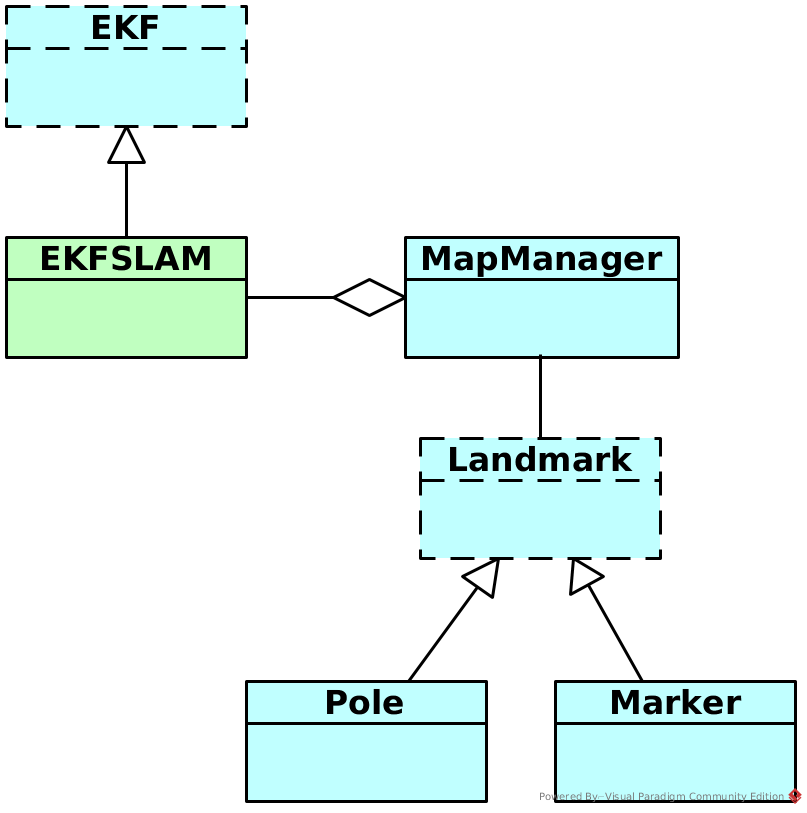
\includegraphics[width=0.5\textwidth]{Images/fig10-class_diagram}
    \caption[Class diagram of the EKFSLAM node]{Class diagram of the EKFSLAM node. The \inlinesrc{EKFSLAM} class is composed by a \inlinesrc{MapManager} instance, which is composed by a list of \inlinesrc{Landmarks}. The \inlinesrc{Landmark} class is abstract and its concrete classes are \inlinesrc{Pole} and \inlinesrc{Marker}.}
    \label{fig:chapter2:architecture:class}
\end{figure}

The main element of the EKF-SLAM node is the \inlinesrc{EKFSLAM} class which is responsible of keeping track of the state vector and execute the EKF-SLAM algorithm. This class inherit from an abstract class called \inlinesrc{EKF}, which is responsible of the implementation of the algorithm in a generic way, while the specifics for the current problem is contained in its child.\\

There are several components that interact within \inlinesrc{EKFSLAM} class, but probably the most interesting one is the \inlinesrc{MapManager} class. This class is responsible of maintaining an updated map of the environment with all the poles and markers, and to save and retrieve the map from a YAML file.\\

The \inlinesrc{MapManager} class contains a list of \inlinesrc{Landmark}s, and every time the state vector is updated in \inlinesrc{EKFSLAM} class, the \inlinesrc{MapManager} class updates the information about each \inlinesrc{Marker}. As mentioned before, the pose of each pole is known and needs no update. Furthermore, the \inlinesrc{Landmark} class is specialized in a \inlinesrc{Marker} class and a \inlinesrc{Pole} class, each of which is responsible of provide the observation model associated to it and the needed Jacobian matrices for the algorithm, hiding the implementation to the \inlinesrc{EKFSLAM} class.
\subsection{ROS nodes}
\label{subsec:chapter2:arch:nodes}
\begin{figure}[h]
    \centering
    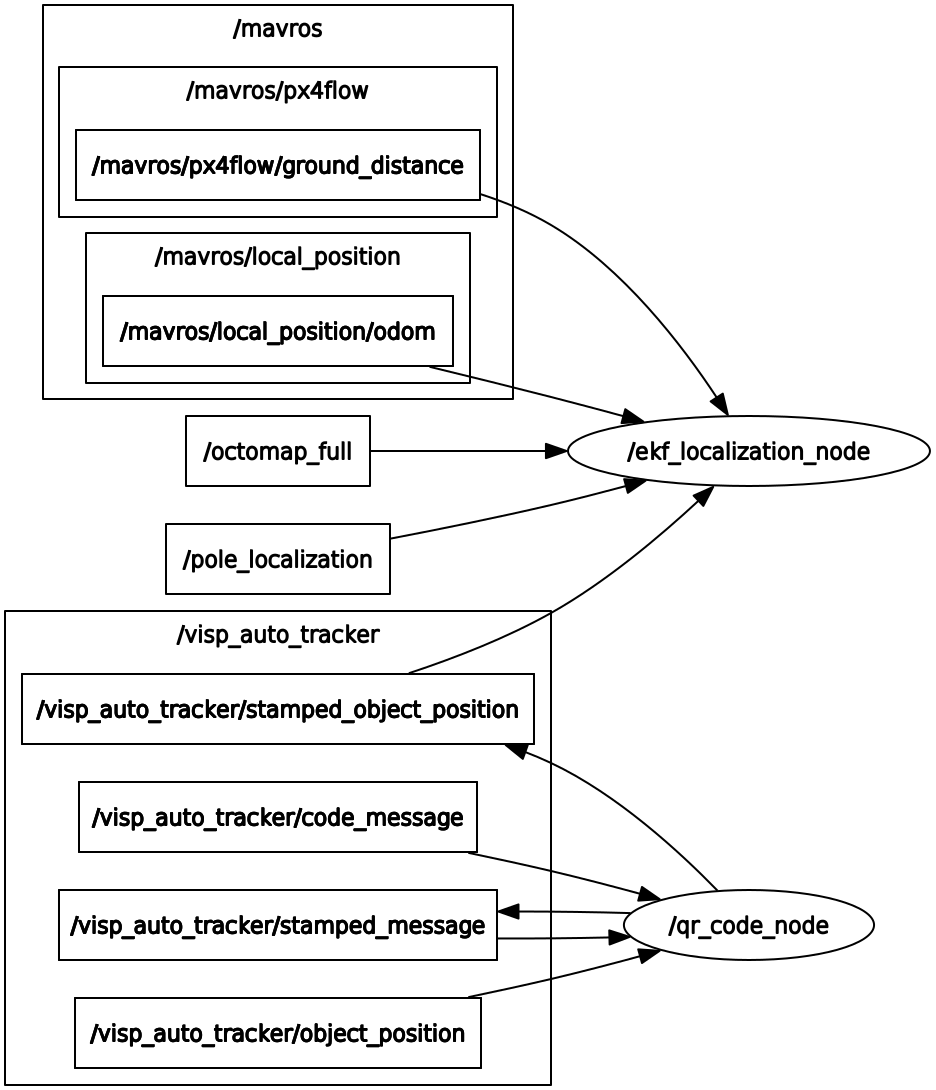
\includegraphics[width=0.8\textwidth]{Images/fig12-rosgraph_ekf_node}
    \caption[Detail of the EKF-SLAM node interactions]{Detail of the EKF-SLAM node interactions. Beside the \inlinesrc{/ekf_localization_node}, the \inlinesrc{/qr_node_code} can be seen. This node, is responsible of subscribing the \inlinesrc{/visp_auto_tracker} messages in order to, then, publish the identifier along with the pose of the marker that has been seen. On the other hand, the \inlinesrc{/ekf_localization_node} subscribes to the \inlinesrc{/mavros}, \inlinesrc{/octomap}, \inlinesrc{/pole_localization} and \inlinesrc{/visp_auto_tracker} messages.}
    \label{fig:chapter2:architecture:nodes:ekf_node}
\end{figure}

Figure~\ref{fig:chapter2:architecture:nodes:ekf_node} shows the detail for the localization node, \inlinesrc{/ekf_localization_node}, with all its subscriptions. It is worth to mention the \inlinesrc{/qr_code_node}, which publishes the markers position with its identifier, subscribes to \inlinesrc{/visp_auto_tracker/code_message} and \inlinesrc{/visp_auto_tracker/object_position}, and publishes into \inlinesrc{/visp_auto_tracker/stamped_object_position} topic.\\

Regarding the \ac{ROS} nodes that comprise the system, in Figure~\ref{fig:chapter2:architecture:nodes:all} all the ones that interact with the localization node and all the others are shown. The EKF-SLAM node, and as mentioned before, interacts with \inlinesrc{/mavros} node, all the poles identification nodes (\inlinesrc{/poles_vision_#}), the \inlinesrc{/qr_code_node}, and the \inlinesrc{/rtabmap} node that provides the Octomap messages. The message passing is represented by arrows, where an incoming arrow means that a node subscribes to the message topic, while an outgoing arrow means that the node publishes that message topic. Arrows go from a node to a topic or from a topic to a node, but do not go from node to node. Its reason lies on the fact that nodes interact between each other using a message passing interface as mention in Section~\ref{sec:chapter1:ros}. Furthermore, it is worth to mention that in Figure~\ref{fig:chapter2:architecture:nodes:all} a \inlinesrc{/gazebo} node is present. This node appears only on simulation and represents the simulated environment, that is why it publishes all the cameras and stereo cameras information.\\
\begin{figure}
    \centering
    \includegraphics[width=\textwidth]{Images/fig11-rosgraph_all}
    \caption[ROS graph of the system]{\ac{ROS} graph of the system. Nodes are depicted as ellipses, while message topics are depicted as boxes. Each arrow means that a node publishes or subscribes to a specific message topic.}
    \label{fig:chapter2:architecture:nodes:all}
\end{figure}




















